\subsection{TCP Vegas}

\subsubsection{Congestion avoidance}

\mKeyword{Reaction to congestion episode} and not to packets loss.
Modifications:
\begin{itemize}
  \item Modified Congestion Avoidance
  \item Aggressive Retransmission
  \item Aggressive Window Adaptation 
  \item Modified SS phase
\end{itemize}

\paragraph*{Congestion Avoidance} It's the reaction per congestion episode not
per loss (congestion control). It uses change in observed end to end delay to
detect onset of congestion, comparing the expected throughput\dots
\begin{equation}
  Expected\ throughput = \frac{window\ size}{RTT}
  \label{eq:tcpvegas:extr}
\end{equation}
\dots and with the actual one:
\begin{equation}
  Actual\ throughput: \frac{actual\ transmitted\ amount}{RTT}
  \label{eq:tcpvegas:actr}
\end{equation}
If there is no congestion, the Actual Throughput will be very close to the
(optimal) Expected Throughput. The difference between Actual Throughput and
Expected Throughput will be greater when there is congestion.\footnote{
  \url{http://www.mathcs.emory.edu/~cheung/Courses/558/Syllabus/02-transport/vegas.html}
}
In this protocol it's important to note that actual throughput can only be equal
or less than expected.
The \mKeyword{monitor transmission rate} is:
\begin{itemize}
\item If $expected - \alpha < actual < expected$: Queues decreasing
  $\rightarrow$ increase transmission rate. $cwnd = \frac{cwnd + 1}{cwnd}$
\item If $expected - \alpha < actual < expected - \beta$: Don’t do anything
\item If $actual < expected - \beta$: Queues increasing $\rightarrow$ decrease
  transmission rate before packet drop (maybe there is a congestion in network
  or maybe the connection is shared among other services).
  $cwnd = \frac{cwnd - 1}{cwnd}$
\end{itemize}

Thresholds of $\alpha = \frac{1 pkts}{RTT}$ and
$\beta = \frac{3 pkts}{RTT}$ correspond to how many packets Vegas is willing
to have in queues.
\begin{figure}[t]
  \centering
  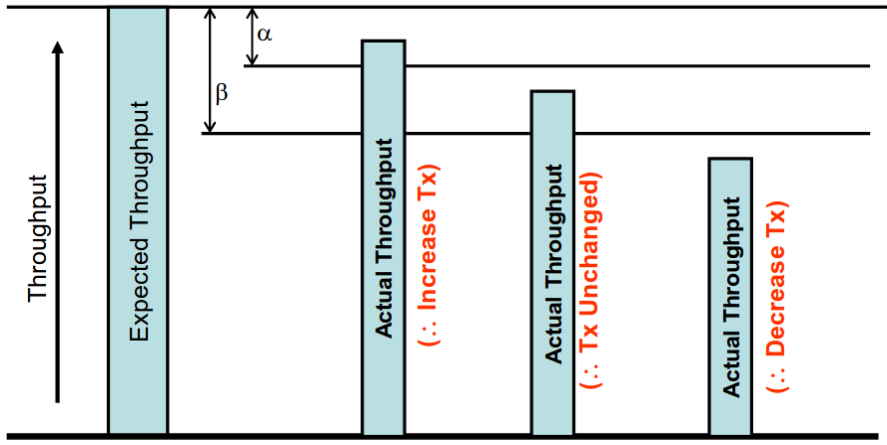
\includegraphics[scale=0.35]{CAVegas}
  \caption{Vegas - Modified Congestion Avoidance}
  \label{fig:tcpVegas:mca}
\end{figure}

There are some definitions to keep in mind: the \mKeyword{throughput} that is
the speed of transmission, and \mKeyword{goodput} that is the speed of reception

\paragraph*{Aggressive Retransmission} With dupacks, when Vegas receives the
first dupack or the second dupacks, it checks the fine grained timer expiry.
This helps in wireless environments with non congestion loss.

\paragraph*{Aggressive Window Adaptation} With recovery, the cwnd is divided by
four instead of two when it enters into recovery. With multiple loss, in case of
multiple segment loss from a single window, it reduces the cwnd only once. The
cwnd is initially set to 2 instead of 1.

\paragraph*{Modified SS phase} The formulas for throughput are the same
of~\ref{eq:tcpvegas:extr} and~\ref{eq:tcpvegas:actr}, but they're calculated in
every alternate RTT instead of once every RTT. There is a new parameter, $\gamma$,
that's calculated as $\gamma = \frac{1pkts}{RTT}$, having that if:
\begin{itemize}
\item $Expected - Actual < \gamma \to$ continue using slow start
\item $Expected - Actual > \gamma \to$ switch to congestion avoidance
\end{itemize}

\begin{figure}[h]
  \centering
  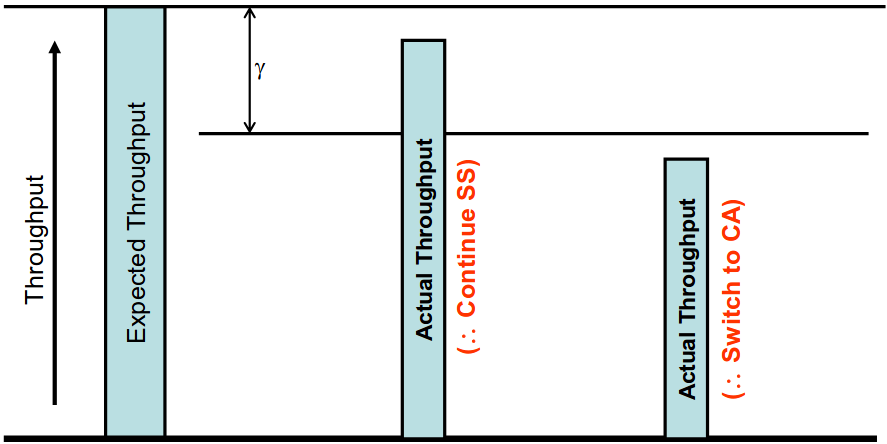
\includegraphics[scale=0.35]{TCPVegasSS}
  \caption{Vegas - Modifies Slow Start}
  \label{fig:tcpvegas:ss}
\end{figure}

\subsubsection{Final considerations}

Unfortunately, TCP Vegas is not actually used: it's sensitive to delay variation
and cannot coexist with legacy TCP versions. At the end of the day, thanks to
its ideas, parts of this protocol have been implemented in other TCP versions.
